\documentclass{standalone}

\usepackage{tikz}
\usetikzlibrary{arrows.meta,angles,quotes,decorations.pathreplacing,positioning}

\usepackage{newtx}
\usepackage{bm}
\renewcommand\mathbf\bm

\begin{document}
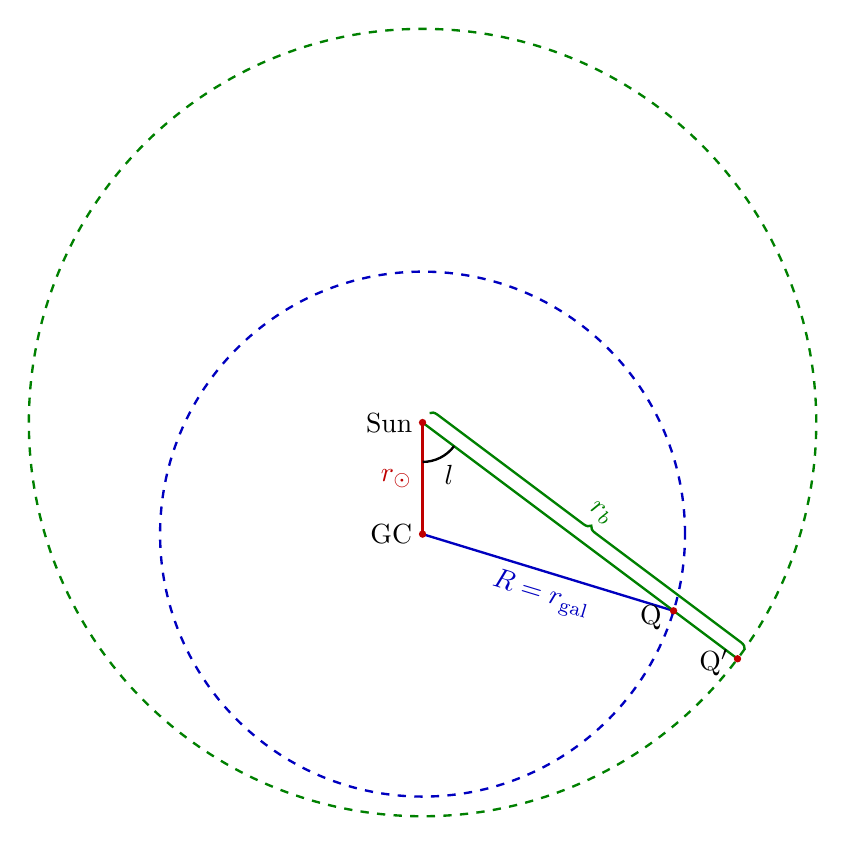
\begin{tikzpicture}[line width=0.3mm,scale=0.6666667]
    \coordinate [label=left:GC] (O) at (0,0);
    \coordinate [label=left:Sun] (S) at (0,2.125);
    \draw [blue!75!black,dashed] (O) circle [radius=5cm];
    \draw [green!50!black,dashed] (S) circle [radius=7.5cm];
    \coordinate (Q') at (6,-2.375);
    \coordinate (Q) at (4.7817017,-1.4612763);
    \draw [red!75!black] (O) -- (S) node [midway,left] {$r_\odot$};
    \draw [blue!75!black] (O) -- (Q) node [midway,below,sloped] {$R=r_{\mathrm{gal}}$};
    \draw [green!50!black] (S) -- (Q');
    \draw [green!50!black,decoration={brace,raise=1.5mm},decorate] (S) -- (Q') node [midway,above=2mm,sloped] {$r_b$};
    \path (O) -- (S) -- (Q) pic ["$l$",draw,angle radius=0.5cm,angle eccentricity=1.5] {angle = O--S--Q};
    \fill [color=red!75!black] (O) circle (2pt);
    \fill [color=red!75!black] (S) circle (2pt);
    \fill [color=red!75!black] (Q) circle (2pt);
    \fill [color=red!75!black] (Q') circle (2pt);
    \node at (5.55,-2.45) {$\mathrm{Q}'$};
    \node at (4.35,-1.6) {Q};
\end{tikzpicture}
\end{document}